\documentclass{standalone}
\usepackage{tikz}
\usepackage{ctex,siunitx}
\usepackage{tkz-euclide}
\usepackage{amsmath}
\usetikzlibrary{patterns, calc}
\usetikzlibrary {decorations.pathmorphing, decorations.pathreplacing, decorations.shapes,}
\begin{document}
\small
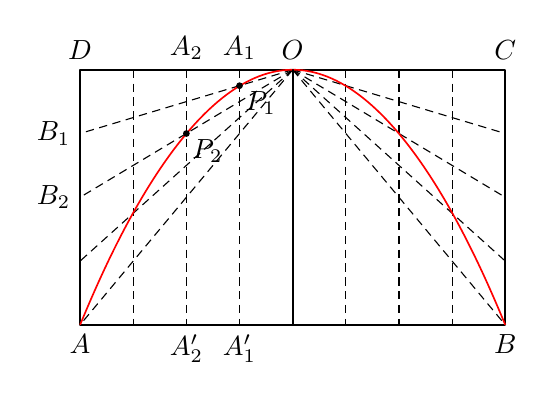
\begin{tikzpicture}[>=latex,scale=0.9]
  \tkzDefPoints{0/0/O,-3/-3.6/A,3/-3.6/B,3/0/C,-3/0/D,0/-3.6/H,-3/-0.9/B1,-3/-1.8/B2,-0.75/0/A1,-1.5/0/A2,-0.75/-3.6/A3,-1.5/-3.6/A4}
  \tkzInterLL(A1,A3)(O,B1)\tkzGetPoint{P1}
  \tkzInterLL(A2,A4)(O,B2)\tkzGetPoint{P2}
  \foreach \x in {0.75,1.5,2.25} 
    {
      \draw[thin,densely dashed](\x,0)--++(0,-3.6);
      \draw[thin,densely dashed](-\x,0)--++(0,-3.6);
    }
  \foreach \x in {1,...,4} 
    {
      \draw[thin,densely dashed] (O)--(-3,-0.9*\x);
      \draw[thin,densely dashed] (O)--(3,-0.9*\x);
    }
  \tkzDrawPolygon[semithick](A,B,C,D)
  \draw[semithick,red](A)parabola bend (O) (B);
  \tkzDrawSegments[semithick](O,H)
  \foreach \x in {1,2}
  {
    \node at (-0.75*\x,0)[above]{$A_\x$};
    \node at (-0.75*\x,-3.6)[below]{$A'_\x$};
    \node at (-3,-0.9*\x)[left]{$B_\x$};
  }
  \tkzDrawPoints[fill=black](P1,P2)
  \tkzLabelPoints[below](A,B)
  \tkzLabelPoint[below right,inner sep=2pt](P1){$P_1$}
  \tkzLabelPoint[below right,inner sep=2pt](P2){$P_2$}
  \tkzLabelPoints[above](O,D,C)
\end{tikzpicture}
\end{document}